\documentclass[a4paper,12pt]{report}

\usepackage{cmap}
\usepackage[T2A]{fontenc}
\usepackage[utf8]{inputenc}
\usepackage[english,russian]{babel}
\usepackage{listings}
\usepackage{amsmath}
\usepackage{float}
\usepackage{csquotes}
\usepackage{mathtools}
\usepackage{hyphenat}
\usepackage{amsfonts}
\usepackage{upgreek}

\usepackage{xcolor}
\usepackage{hyperref}

\usepackage{graphicx}
\graphicspath{ {./images/} }

\definecolor{dkgreen}{rgb}{0,0.6,0}
\definecolor{gray}{rgb}{0.5,0.5,0.5}
\definecolor{mauve}{rgb}{0.58,0,0.82}

\lstset{
    language=Python,                 % выбор языка для подсветки (здесь это С)
    basicstyle=\small\sffamily, % размер и начертание шрифта для подсветки кода
    numbers=left,               % где поставить нумерацию строк (слева\справа)
    numberstyle=\tiny,           % размер шрифта для номеров строк
    stepnumber=1,                   % размер шага между двумя номерами строк
    numbersep=5pt,                % как далеко отстоят номера строк от подсвечиваемого кода
    aboveskip=3mm,
    belowskip=3mm,
    showstringspaces=false,
    columns=flexible,
    captionpos=b, 
    basicstyle={\small\ttfamily},
    numbers=left,
    numberstyle=\tiny\color{gray},
    keywordstyle=\color{blue},
    commentstyle=\color{mauve},
    stringstyle=\color{dkgreen},
    breaklines=true,
    breakatwhitespace=true,
    tabsize=3
}

\title{Лабораторная работа №9\\Дифференцирование и интегрирование}
\author{Кобыжев Александр}
\date{\today}

\begin{document}

\maketitle
\tableofcontents
\listoffigures
\lstlistoflistings

\maketitle

\chapter{Упражнение 9.1}

В данном упражнении нас просят открыть \texttt{chap09.ipynb}, прочитать пояснения, а также запустить примеры. 

\chapter{Упражнение 9.2}

Создадим волну \texttt{TriangleSignal}:

\begin{lstlisting}[caption=Создание треугольного сигнала]
in_wave = thinkdsp.TriangleSignal(freq=50).make_wave(duration=0.1, framerate=44000)
in_wave.plot()
thinkplot.config(xlabel='Time (s)')
\end{lstlisting}

\begin{figure}[H]
        \centering
        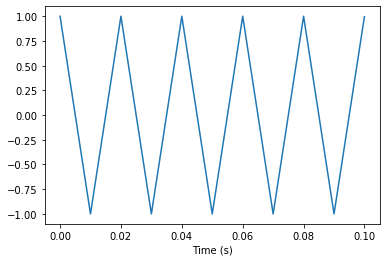
\includegraphics[width=0.75\textwidth]{lab9_fig2_1.png}
        \caption{Визуализация треугольного сигнала}
        \label{fig:lab9_fig2_1}
\end{figure}

\texttt{diff} треугольной волны - это прямоугольная волна, что объясняет, почему гармоники в прямоугольной волне уменьшаются как $1/f$, по сравнению с треугольной волной, которая спадает как $1/f2$.

\begin{lstlisting}[caption=Визуализация при \texttt{diff}]
out_wave = in_wave.diff()
out_wave.plot()
thinkplot.config(xlabel='Time (s)')
\end{lstlisting}

\begin{figure}[H]
        \centering
        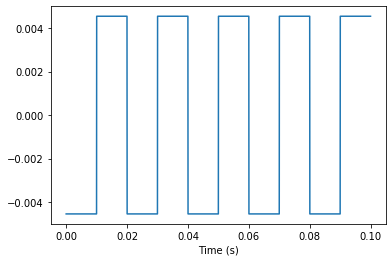
\includegraphics[width=0.75\textwidth]{lab9_fig2_2.png}
        \caption{Визуализация при \texttt{diff}}
        \label{fig:lab9_fig2_2}
\end{figure}

Когда мы берём спектральную производную, мы получаем "звон" вокруг разрывов:

\begin{lstlisting}[caption=Визуализация при \texttt{differentiate}]
out_wave2 = in_wave.make_spectrum().differentiate().make_wave()
out_wave2.plot()
thinkplot.config(xlabel='Time (s)')
\end{lstlisting}

\begin{figure}[H]
        \centering
        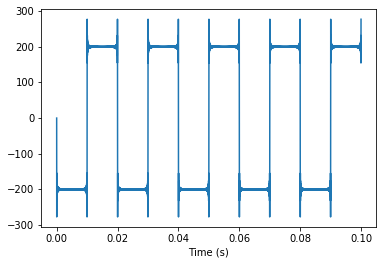
\includegraphics[width=0.75\textwidth]{lab9_fig2_3.png}
        \caption{Визуализация при \texttt{differentiate}}
        \label{fig:lab9_fig2_3}
\end{figure}

Различия между эффектом \texttt{diff} и \texttt{differentiate} заключается в том, что производная треугольной волны не определена в точках треугольника.

\chapter{Упражнение 9.3}

Сделаем волну \texttt{SquareSignal}:

\begin{lstlisting}[caption=Создание сигнала]
in_wave = thinkdsp.SquareSignal(freq=50).make_wave(duration=0.1, framerate=44000)
in_wave.plot()
thinkplot.config(xlabel='Time (s)')
\end{lstlisting}

\begin{figure}[H]
        \centering
        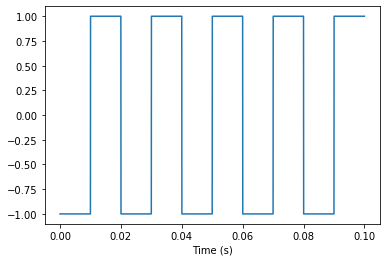
\includegraphics[width=0.75\textwidth]{lab9_fig3_1.png}
        \caption{Визуализация сигнала}
        \label{fig:lab9_fig3_1}
\end{figure}

Совокупная сумма прямоугольной волны - это треугольная волна. После предыдущего выполненного упражнения это не должно вызывать никакого удивления.

\begin{lstlisting}[caption=Визуализация при \texttt{cumsum}]
out_wave = in_wave.cumsum()
out_wave.plot()
thinkplot.config(xlabel='Time (s)')
\end{lstlisting}

\begin{figure}[H]
        \centering
        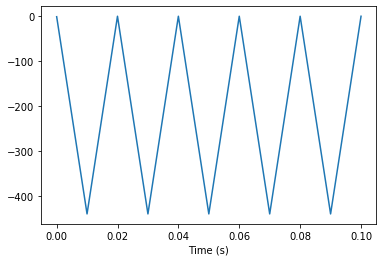
\includegraphics[width=0.75\textwidth]{lab9_fig3_2.png}
        \caption{Визуализация при \texttt{cumsum}}
        \label{fig:lab9_fig3_2}
\end{figure}

Спектральный интеграл также представляет собой треугольную волну, хотя амплитуда сильно отличается.

\begin{lstlisting}[caption=Визуализация при \texttt{integrate}]
spectrum = in_wave.make_spectrum().integrate()
spectrum.hs[0] = 0
out_wave2 = spectrum.make_wave()
out_wave2.plot()
thinkplot.config(xlabel='Time (s)')
\end{lstlisting}

\begin{figure}[H]
        \centering
        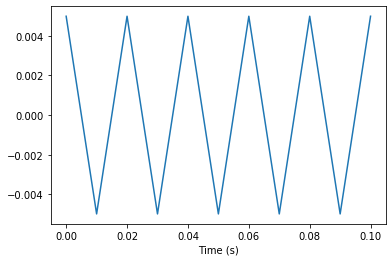
\includegraphics[width=0.75\textwidth]{lab9_fig3_3.png}
        \caption{Визуализация при \texttt{integrate}}
        \label{fig:lab9_fig3_3}
\end{figure}

Если уравновесить и нормализовать две волны, они будут визуально похожи.

\begin{lstlisting}[caption=Сравнение волн]
out_wave.unbias()
out_wave.normalize()
out_wave2.normalize()
out_wave.plot()
out_wave2.plot()
\end{lstlisting}

\begin{figure}[H]
        \centering
        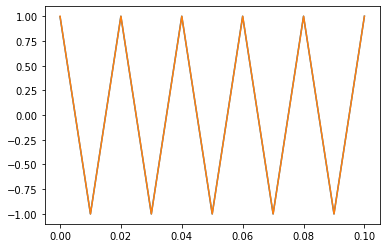
\includegraphics[width=0.75\textwidth]{lab9_fig3_4.png}
        \caption{Сравнение волн}
        \label{fig:lab9_fig3_4}
\end{figure}

\begin{lstlisting}[caption=Разница между реализациями]
max(abs(out_wave.ys - out_wave2.ys))
\end{lstlisting}

Разница составила \texttt{0.004545454545454519}. Они численно похожи, но с точностью около 3 цифр.

\chapter{Упражнение 9.4}

Создадим \texttt{SawtoothSignal} волну.

\begin{lstlisting}[caption=Создание сигнала]
in_wave = thinkdsp.SawtoothSignal(freq=50).make_wave(duration=0.1, framerate=44000)
in_wave.plot()
thinkplot.config(xlabel='Time (s)')
\end{lstlisting}

\begin{figure}[H]
        \centering
        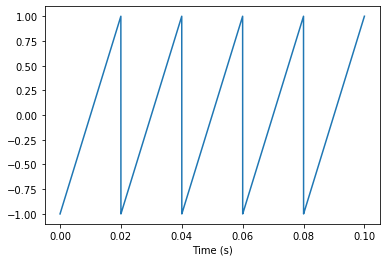
\includegraphics[width=0.75\textwidth]{lab9_fig4_1.png}
        \caption{Создание сигнала}
        \label{fig:lab9_fig4_1}
\end{figure}

Первая совокупная сумма зубца пилы - это парабола:

\begin{lstlisting}[caption=Первая совокупная сумма]
out_wave = in_wave.cumsum()
out_wave.unbias()
out_wave.plot()
thinkplot.config(xlabel='Time (s)')
\end{lstlisting}

\begin{figure}[H]
        \centering
        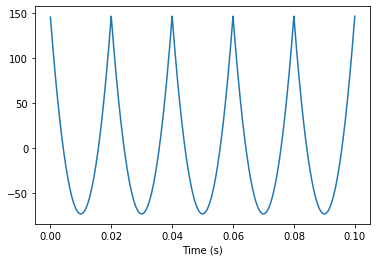
\includegraphics[width=0.75\textwidth]{lab9_fig4_2.png}
        \caption{Первая совокупная сумма}
        \label{fig:lab9_fig4_2}
\end{figure}

Вторая совокупная сумма - это кубическая кривая:

\begin{lstlisting}[caption=Вторая совокупная сумма]
out_wave = out_wave.cumsum()
out_wave.plot()
thinkplot.config(xlabel='Time (s)')
\end{lstlisting}

\begin{figure}[H]
        \centering
        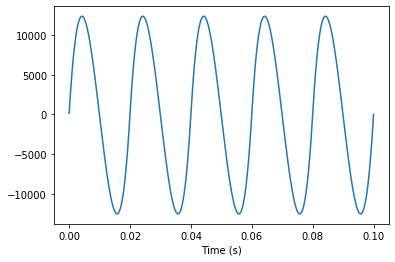
\includegraphics[width=0.75\textwidth]{lab9_fig4_3.png}
        \caption{Вторая совокупная сумма}
        \label{fig:lab9_fig4_3}
\end{figure}

Двойное интегрирование также дает кубическую кривую.

\begin{lstlisting}[caption=Двойное интегрирование]
spectrum = in_wave.make_spectrum().integrate().integrate()
spectrum.hs[0] = 0
out_wave2 = spectrum.make_wave()
out_wave2.plot()
thinkplot.config(xlabel='Time (s)')
\end{lstlisting}

\begin{figure}[H]
        \centering
        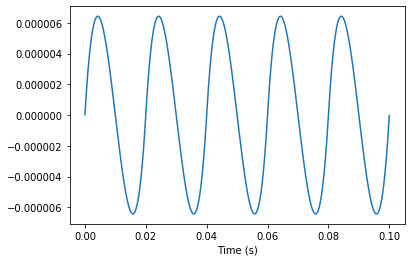
\includegraphics[width=0.75\textwidth]{lab9_fig4_4.png}
        \caption{Двойное интегрирование}
        \label{fig:lab9_fig4_4}
\end{figure}

На этом этапе результат всё больше и больше напоминает синусоиду. Причина в том, что интеграция действует как фильтр нижних частот. На данный момент мы отфильтровали почти все, кроме основного, как показано в спектре ниже:

\begin{lstlisting}[caption=Спектр сигнала]
out_wave2.make_spectrum().plot(high=500)
\end{lstlisting}

\begin{figure}[H]
        \centering
        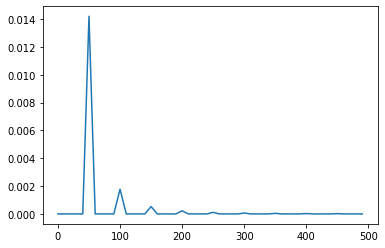
\includegraphics[width=0.75\textwidth]{lab9_fig4_5.png}
        \caption{Спектр сигнала}
        \label{fig:lab9_fig4_5}
\end{figure}

\chapter{Упражнение 9.5}

Создадим волну \texttt{CubicSignal}:

\begin{lstlisting}[caption=Создание сигнала]
in_wave = thinkdsp.CubicSignal(freq=0.0005).make_wave(duration=10000, framerate=1)
in_wave.plot()
\end{lstlisting}

\begin{figure}[H]
        \centering
        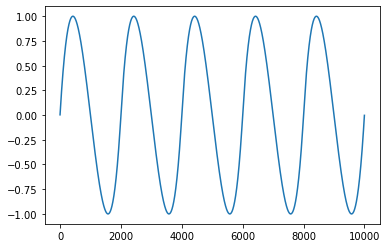
\includegraphics[width=0.75\textwidth]{lab9_fig5_1.png}
        \caption{Создание сигнала}
        \label{fig:lab9_fig5_1}
\end{figure}

Первый \texttt{diff} - парабола, второй - пилообразная волна:

\begin{lstlisting}[caption=Первый \texttt{diff}]
out_wave = in_wave.diff()
out_wave.plot()
\end{lstlisting}

\begin{figure}[H]
        \centering
        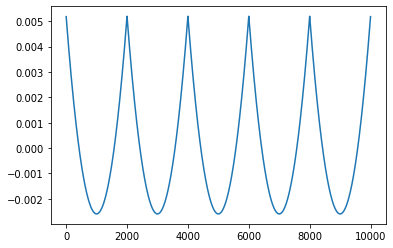
\includegraphics[width=0.75\textwidth]{lab9_fig5_2.png}
        \caption{Первый \texttt{diff}}
        \label{fig:lab9_fig5_2}
\end{figure}

\begin{lstlisting}[caption=Второй \texttt{diff}]
out_wave = out_wave.diff()
out_wave.plot()
\end{lstlisting}

\begin{figure}[H]
        \centering
        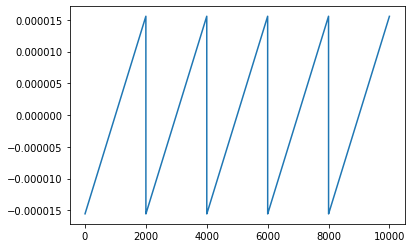
\includegraphics[width=0.75\textwidth]{lab9_fig5_3.png}
        \caption{Второй \texttt{diff}}
        \label{fig:lab9_fig5_3}
\end{figure}

Когда мы дифференцируем дважды, получаем пилообразную форму с некоторым звоном. Проблема в том, что производная параболического сигнала в точках не определена.

\begin{lstlisting}[caption=Вторая производная]
spectrum = in_wave.make_spectrum().differentiate().differentiate()
out_wave2 = spectrum.make_wave()
out_wave2.plot()
thinkplot.config(xlabel='Time (s)')
\end{lstlisting}

\begin{figure}[H]
        \centering
        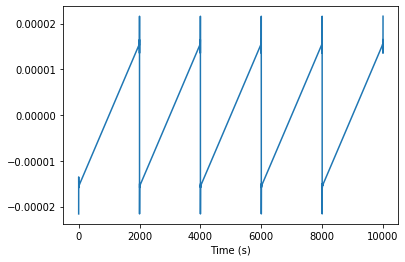
\includegraphics[width=0.75\textwidth]{lab9_fig5_4.png}
        \caption{Вторая производная}
        \label{fig:lab9_fig5_4}
\end{figure}

Окно второй разности -1, 2, -1. Вычисляя ДПФ окна, мы можем найти соответствующий фильтр.

\begin{lstlisting}[caption=ДПФ окна]
diff_window = np.array([-1.0, 2.0, -1.0])
padded = thinkdsp.zero_pad(diff_window, len(in_wave))
diff_wave = thinkdsp.Wave(padded, framerate=in_wave.framerate)
diff_filter = diff_wave.make_spectrum()
diff_filter.plot(label='2nd diff')

thinkplot.config(xlabel='Frequency (Hz)',
                 ylabel='Amplitude ratio',
                 loc='lower right')
\end{lstlisting}

\begin{figure}[H]
        \centering
        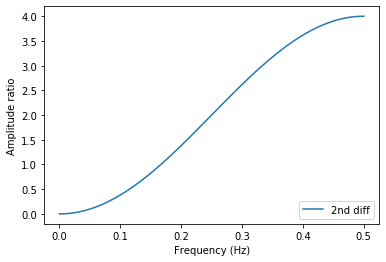
\includegraphics[width=0.75\textwidth]{lab9_fig5_5.png}
        \caption{ДПФ окна}
        \label{fig:lab9_fig5_5}
\end{figure}

А для второй производной мы можем найти соответствующий фильтр, вычислив фильтр первой производной и возведя его в квадрат.

\begin{lstlisting}[caption=Фильтр второй производной]
deriv_filter = in_wave.make_spectrum()
deriv_filter.hs = (PI2 * 1j * deriv_filter.fs)**2
deriv_filter.plot(label='2nd deriv')

thinkplot.config(xlabel='Frequency (Hz)',
                 ylabel='Amplitude ratio',
                 loc='lower right')
\end{lstlisting}

\begin{figure}[H]
        \centering
        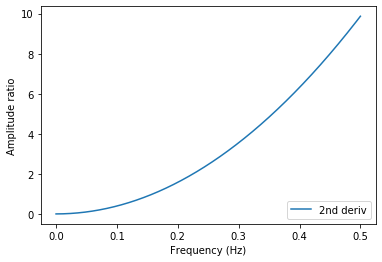
\includegraphics[width=0.75\textwidth]{lab9_fig5_6.png}
        \caption{Фильтр второй производной}
        \label{fig:lab9_fig5_6}
\end{figure}

Рассмотрим два фильтра в одном масштабе:

\begin{lstlisting}[caption=Визуализация двух фильтров]
diff_filter.plot(label='2nd diff')
deriv_filter.plot(label='2nd deriv')

thinkplot.config(xlabel='Frequency (Hz)',
                 ylabel='Amplitude ratio',
                 loc='lower right')
\end{lstlisting}

\begin{figure}[H]
        \centering
        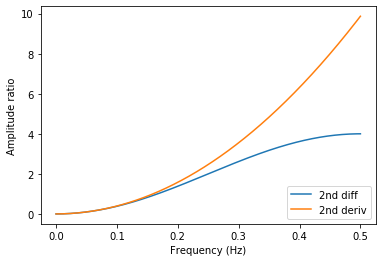
\includegraphics[width=0.75\textwidth]{lab9_fig5_7.png}
        \caption{Визуализация двух фильтров}
        \label{fig:lab9_fig5_7}
\end{figure}

Теперь мы можем видеть, что оба являются фильтрами верхних частот, которые усиливают компоненты самых высоких частот. Второй \texttt{deriv} параболический, поэтому он сильнее всего усиливает самые высокие частоты. Второй \texttt{diff} - хорошее приближение второй производной только на самых низких частотах, затем он существенно отклоняется.

\chapter{Выводы}

Во время выполнения лабораторной работы получены навыки работы с взаимосвязью между окнами во временной области и фильтрами в частотной области. Также изучалось влияние окна конечных разностей, которое приближает дифференцирование, и операции накопления суммы, которая приближает интегрирование.

\end{document}